% Version 0; outline format; Written by SH

%% ------------------------------------------------------------------------------------ %% 
\documentclass[a4paper,fleqn,usenatbib]{mnras}

% Packages
\usepackage{deluxetable}
\usepackage{newtxtext,newtxmath}
\usepackage[T1]{fontenc}
\usepackage{ae,aecompl}
\usepackage{amssymb, amsmath}
\usepackage{graphicx}
\usepackage{natbib}
\usepackage{url}
\usepackage{hyperref}
\usepackage{float}
\usepackage[usenames, dvipsnames]{color}

% Package Settings
\hypersetup{colorlinks=true,
            citecolor=MidnightBlue,
            linkcolor=MidnightBlue,
            filecolor=magenta,      
            urlcolor=cyan}
\urlstyle{same}

% Figure extention
\DeclareGraphicsExtensions{.pdf,.png,.jpg}

%% ------------------------------------------------------------------------------------ %% 
%% ---------------------------- User Defined Commands --------------------------------- %%
%% ------------------------------------------------------------------------------------ %% 

% Song Huang's definition 
\def\arcsec{{\prime\prime}}
\def\arcmin{{\prime}}
\def\degree{{\circ}}
\def\h{\hskip -3 mm}
\def\aa{{A\&A}}
\def\aas{{ A\&AS}}
\def\aj{{AJ}}
\def\al{$\alpha$}
\def\bet{$\beta$}
\def\amin{$^\prime$}
\def\annrev{{ARA\&A}}
\def\apj{{ApJ}}
\def\apjs{{ApJS}}
\def\asec{$^{\prime\prime}$}
\def\deg{$^{\circ}$}
\def\ddeg{{\rlap.}$^{\circ}$}
\def\dsec{{\rlap.}$^{\prime\prime}$}
\def\cc{cm$^{-3}$}
\def\flamb{erg s$^{-1}$ cm$^{-2}$ \AA$^{-1}$}
\def\flux{erg s$^{-1}$ cm$^{-2}$}
\def\fnu{erg s$^{-1}$ cm$^{-2}$ Hz$^{-1}$}
\def\hst{{\textit{HST}}}
\def\kms{km s$^{-1}$}
\def\lamb{$\lambda$}
\def\lax{{$\mathrel{\hbox{\rlap{\hbox{\lower4pt\hbox{$\sim$}}}\hbox{$<$}}}$}}
\def\gax{{$\mathrel{\hbox{\rlap{\hbox{\lower4pt\hbox{$\sim$}}}\hbox{$>$}}}$}}
\def\simlt{\lower.5ex\hbox{$\; \buildrel < \over \sim \;$}}
\def\simgt{\lower.5ex\hbox{$\; \buildrel > \over \sim \;$}}
\def\micron{{$\mu$m}}
\def\mnras{{MNRAS}}
\def\nat{{Nature}}
\def\pasp{{PASP}}
\def\perang{\AA$^{-1}$}
\def\peryr{yr$^{-1}$}
\def\reference{\noindent\pp}
\def\refindent{\par\noindent\parskip=2pt\hangindent=3pc\hangafter=1 }
\def\sb{mag~arcsec$^{-2}$}
\def\lsun{$L_\odot$} 
\def\msun{$M_\odot$}
\def\sigs{$\sigma_*$}
\newcommand{\lt}{<}
\newcommand{\gt}{>}

\def\etal{{\ et al.~}}
\def\galfit{{\tt GALFIT}}
\def\ser{{S\'{e}rsic\ }}
\def\redm{\texttt{redMaPPer}}
\def\cmodel{\texttt{cModel}}

% Samples
\def\rbcg{\texttt{cenHighMh}}
\def\nbcg{\texttt{cenLowMh}}
\def\redbcg{{$\lambda \ge 30$}}
\def\nonbcg{{$\lambda < 20$}}

% Mass related 
\def\mstar{{$M_{\star}$}}
\def\mhalo{{$M_{\mathrm{halo}}$}}
\def\logms{{$\log (M_{\star}/M_{\odot})$}}
\def\logmh{{$\log (M_{\mathrm{halo}}/M_{\odot})$}}

\def\mA{{$M_{\star,10\ \mathrm{kpc}}$}}
\def\mB{{$M_{\star,30\ \mathrm{kpc}}$}}
\def\mC{{$M_{\star,50\ \mathrm{kpc}}$}}
\def\mD{{$M_{\star,100\ \mathrm{kpc}}$}}
\def\mtot{{$M_{\star,\mathrm{Tot}}$}}
\def\minn{{$M_{\star,10\ \mathrm{kpc}}$}}
\def\meff{{$M_{\star,15\ \mathrm{kpc}}$}} 
\def\mout{{$M_{\star,150\ \mathrm{kpc}}$}}
\def\mmax{{$M_{\star,\mathrm{Max}}$}}
\def\mgama{{$M_{\star,\mathrm{GAMA}}$}}
\def\mcmodel{{$M_{\star,\mathrm{cModel}}$}}
\def\msim{{$M_{\star,\mathrm{3D}}$}}

\def\logminn{{$\log (M_{\star,10\ \mathrm{kpc}}/M_{\odot})$}}
\def\logmout{{$\log (M_{\star,150\ \mathrm{kpc}}/M_{\odot})$}}
\def\logmmax{{$\log (M_{\star,\mathrm{Max}}/M_{\odot})$}}
\def\logmgama{{$\log (M_{\star,\mathrm{GAMA}}/M_{\odot})$}}
\def\logmcmodel{{$\log (M_{\star,\mathrm{cModel}}/M_{\odot})$}}
\def\logm10{{$\log (M_{\star,10\ \mathrm{kpc}}/M_{\odot})$}}
\def\logm30{{$\log (M_{\star,30\ \mathrm{kpc}}/M_{\odot})$}}
\def\logm50{{$\log (M_{\star,50\ \mathrm{kpc}}/M_{\odot})$}}
\def\logm100{{$\log (M_{\star,100\ \mathrm{kpc}}/M_{\odot})$}}
\def\logmtot{{$\log (M_{\star,\mathrm{Tot}}/M_{\odot})$}}
\def\logmsim{{$\log (M_{\star,\mathrm{3D}}/M_{\odot})$}}

\def\mvir{{$M_{\mathrm{Halo,\ Vir}}$}}
\def\mpeak{{$M_{\mathrm{Halo,\ Peak}}$}}
\def\mall{{$M_{\star,\mathrm{All}}$}}
\def\mbcg{{$M_{\star,\mathrm{BCG}}$}}
\def\micl{{$M_{\star,\mathrm{ICL}}$}}
\def\mcen{{$M_{\star,\mathrm{Cen}}$}}
\def\mgal{{$M_{\star,\mathrm{Gal}}$}}

\def\fraccen{{$M_{\star,\ \mathrm{Cen,\ Ori}} / M_{\star,\ \mathrm{All,\ Ori}}$}}
\def\fracbcg{{$M_{\star,\ \mathrm{BCG,\ Ori}} / M_{\star,\ \mathrm{Cen,\ Ori}}$}}
\def\fracins{{$M_{\star,\ \mathrm{in-situ,\ Ori}} / M_{\star,\ \mathrm{Cen,\ Ori}}$}}

\def\sigms{{$\sigma_{\log\ M_{\star}}$}}
\def\sigmh{{$\sigma_{\log\ M_{\mathrm{Halo}}}$}}

\def\zform{{$z_{\mathrm{form}}$}}
\def\zstarve{{$z_{\mathrm{form}}$}}

\def\m2l{{$M_{\star}/L_{\star}$}}
\def\mden{{$\mu_{\star}$}}

\def\um{\texttt{UniverseMachine}}
\def\htools{\texttt{halotools}}

\def\insitu{\textit{in situ}}
\def\exsitu{\textit{ex situ}}

\def\mins{{$M_{\star,ins}$}}
\def\macc{{$M_{\star,exs}$}}

%% ------------------------------------------------------------------------------------ %% 
% Commenting:
\newcommand{\xxx}[1]{\textcolor{red}{\textbf{XXX}}}
\newcommand{\todo}[1]{\textcolor{blue}{\textbf{TODO:~#1}}}
\newcommand{\plan}[1]{\textcolor{blue}{#1}}
\newcommand{\addref}{{\textcolor{red}{REF}}}
\newcommand{\note}[2]{\textcolor{blue}{\textbf{[Comment (#1): #2]}}}
\newcommand{\song}[1]{\textcolor{cyan}{\textbf{[Song: #1]}}}
\newcommand{\alexie}[1]{\textcolor{Bittersweet}{\textbf{[Alexie: #1]}}}
\newcommand{\question}[1]{\textcolor{Red}{\textbf{[Question: #1]}}}
\newcommand{\update}[1]{\textcolor{Bittersweet}{#1}}

%% ------------------------------------------------------------------------------------ %% 
%% --------------------------- Title and Affiliations --------------------------------- %% 
%% ------------------------------------------------------------------------------------ %% 

\title[Structure of Massive Galaxy and Halo Mass]{The Structure of Massive Galaxies 
    and Its Dependence on Dark Matter Halo Mass}

\author[S. Huang et al.]{
        Song Huang$^{1,2}$\thanks{E-mail: shuang89@ucsc.edu (SH)},
        Alexie Leauthaud$^{1}$,
        Andrew Hearin$^{3}$,
        Peter Behroozi$^{4}$,
        \newauthor
        HSC Collaboration
        \\
        $^{1}$Department of Astronomy and Astrophysics, University of California 
              Santa Cruz, 1156 High St., Santa Cruz, CA 95064, U.S.A\\
        $^{2}$Kavli-IPMU, The University of Tokyo Institutes for Advanced Study, 
              the University of Tokyo (Kavli IPMU, WPI), Kashiwa 277--8583, Japan\\              
        $^{3}$Argonne National Laboratory\\
        $^{4}$University of Arizona
        }   
        
%% ------------------------------------------------------------------------------------ %% 
\date{Accepted XXX. Received YYY; in original form ZZZ}        
\pubyear{2017}                                  

%% ------------------------------------------------------------------------------------ %% 
\begin{document}

\label{firstpage}
\pagerange{\pageref{firstpage}--\pageref{lastpage}}

\maketitle

%% ------------------------------------------------------------------------------------ %% 
%% ------------------------------- Abstract and Keywords ------------------------------ %% 
%% ------------------------------------------------------------------------------------ %% 
\begin{abstract}
    
    \song{Placeholder}
    \plan{
    Using deep images from the Hyper Suprime--Cam (HSC) Survey, we show that the 
    massive central galaxies in less and more massive dark matter halos have different 
    stellar mass distributions. 
    In this work, we use weak lensing (WL) analysis based on HSC images to further 
    investigate the connection between stellar mass distribution and the dark matter 
    halo properties in massive galaxies. 
    We detect a significant dependence that suggest XXXXXXX.
    We also find similar trends in hydrodynamic simulations and semi-empirical models. 
    With the help from the recent \um{} semi-empirical model, we forward modeling the 
    observed stellar mass functions (SMF) for different aperture masses and the WL
    profiles across the \mtot{}-\minn{} plane at the same time. 
    This model provides us a new window to look into the connection between the 
    assembly of massive galaxies and their dark matter haloes. 
    We find XXXXX (put the amazing results here). 
    }

\end{abstract}

\begin{keywords}
    galaxies: evolution --
    galaxies: haloes --
    dark matter --
    surveys
\end{keywords}

%% ------------------------------------------------------------------------------------ %% 
%% ------------------------------------ Main Text ------------------------------------- %% 
%% ------------------------------------------------------------------------------------ %% 

%% ------------------------------------------------------------------------------------ %% 
\section{Introduction}
    \label{sec:intro}

	\plan{Scientific background on galaxy-halo connection for massive galaxies and 
	      why it is important}
	 
	\plan{Motivation: We find that central galaxies in more or less massive dark 
	      matter haloes could have different stellar mass distributions. 
	      This result has many exciting implications about the assembly of massive 
	      galaxies and their galaxy--halo connection. 
	      Here we use the stellar mass distributions of $z~0.4$ massive galaxies 
	      and their weak lensing signals to further study how exactly the dark 
	      matter halo masses connect to the stellar mass within different regions 
	      of massive galaxies. 
	      }
    
%% ------------------------------------------------------------------------------------ %%     
    \song{Placeholder} 
    This paper is organized as follows. 
    \S \ref{sec:data} presents our data and our sample selection. 
    \S \ref{sec:model} describes the \um{} model and how we use it to study the 
    dark matter halo mass across the \mtot{}-\minn{} plane. 
    Our main results are presented in \S \ref{sec:result} and discussed in 
    \S \ref{sec:discussion}. 
    \S \ref{sec:summary} presents our summary and conclusions.

    Magnitudes use the AB system (\citealt{Oke1983}), and are corrected for Galactic 
    extinction using calibrations from \citet{Schlafly11}.
    In this work, we assume $H_0$ = 70~km~s$^{-1}$ Mpc$^{-1}$, ${\Omega}_{\rm m}=0.3$, 
    and ${\Omega}_{\rm \Lambda}=0.7$.
    Stellar mass is noted \mstar{} and has been derived using a Chabrier Initial Mass 
    Function (IMF; \citealt{Chabrier2003}).     
    $M_{\mathrm{halo}}$ denotes halo mass in general whereas $M_{\rm 200b}$ is 
    explicitly defined as $M_{\rm 200b}\equiv M(<r_{\rm 200b})=200\bar{\rho} 
    \times \frac{4}{3}\pi r_{\rm 200b}^3$ where $r_{\rm 200b}$
    is the radius at which the mean interior density is equal to 200 times
    the mean matter density ($\bar{\rho}$). 
    
%% ------------------------------------------------------------------------------------ %% 

%% ------------------------------------------------------------------------------------ %% 
\section{Massive Galaxies observed by Hyper Suprime-Cam Survey}
    \label{sec:data}
    
%% ------------------------------------------------------------------------------------ %% 
\subsection{Sample selection}
    \label{ssec:sample}
    
    \song{Placeholder}
    The Subaru Strategic Program (SSP, \citealt{MiyazakiInPrep}) makes use of the new 
    prime-focus camera, the Hyper Suprime-Cam (HSC;~\citealt{Miyazaki2012}), on the 
    8.2-m Subaru telescope at Mauna Kea. 
    The ambitious multi-layer HSC survey takes advantage of the large field of 
    view (FoV;~1.5 deg in diameter) of this camera and will cover $\sim 1400$ deg$^2$ 
    in 5 broad bands ($grizY$) to a limiting depth of $r \sim 26$ mag 
    in the \texttt{WIDE} layer. 
    This work is based on the internal data release \texttt{S15B}, which covers 
    $\sim 100$ deg$^2$ in all 5-band to full \texttt{WIDE} depth.  
    The regions covered by this release overlap with a number of spectroscopic surveys 
    (e.g.\ SDSS/BOSS: \citealt{Eisenstein2011}, \citealt{Alam2015}; 
    GAMA: \citealt{Driver2011}, \citealt{Liske2015}).

    The HSC \texttt{WIDE} survey is about $3.0$-$4.0$ magnitudes deeper in the $i$-band 
    than SDSS. 
    Combined with the excellent imaging resolution (the median $i$-band seeing is 0.6"), 
    and the wide area, the HSC survey represents a tremendous data set to perform a 
    large statistical study of the surface brightness profiles of ETGs out to large radii.     
    Fig~\ref{fig:sdss_compare} illustrates the quality of HSC imaging compared to SDSS 
    for three low redshift ETGs, and shows that HSC survey data are well suited for 
    mapping the stellar distribution of massive galaxies out to large radii.

	HSC $i$-band images typically have the best seeing compared to other bands because 
	of strict requirements driven by weak lensing science. 
    We will therefore use the $i$-band images to measure the stellar distributions of 
    massive galaxies.
     
%% ------------------------------------------------------------------------------------ %% 
\subsection{Surface mass density profiles and aperture masses}
    \label{ssec:mass}
    
    \plan{Briefly explain how 1-D mass density profiles are extracted and how 
          aperture masses are measured.}
          
%% ------------------------------------------------------------------------------------ %% 
\subsection{Weak lensing analysis around massive galaxies}
    \label{ssec:wl}
    
    \plan{Briefly explain how weak lensing density profiles are measured using HSC 
          images.}

%% ------------------------------------------------------------------------------------ %% 

%% ------------------------------------------------------------------------------------ %% 
\section{Model}
    \label{sec:model}

%% ------------------------------------------------------------------------------------ %% 
    \begin{figure*}
        \centering 
        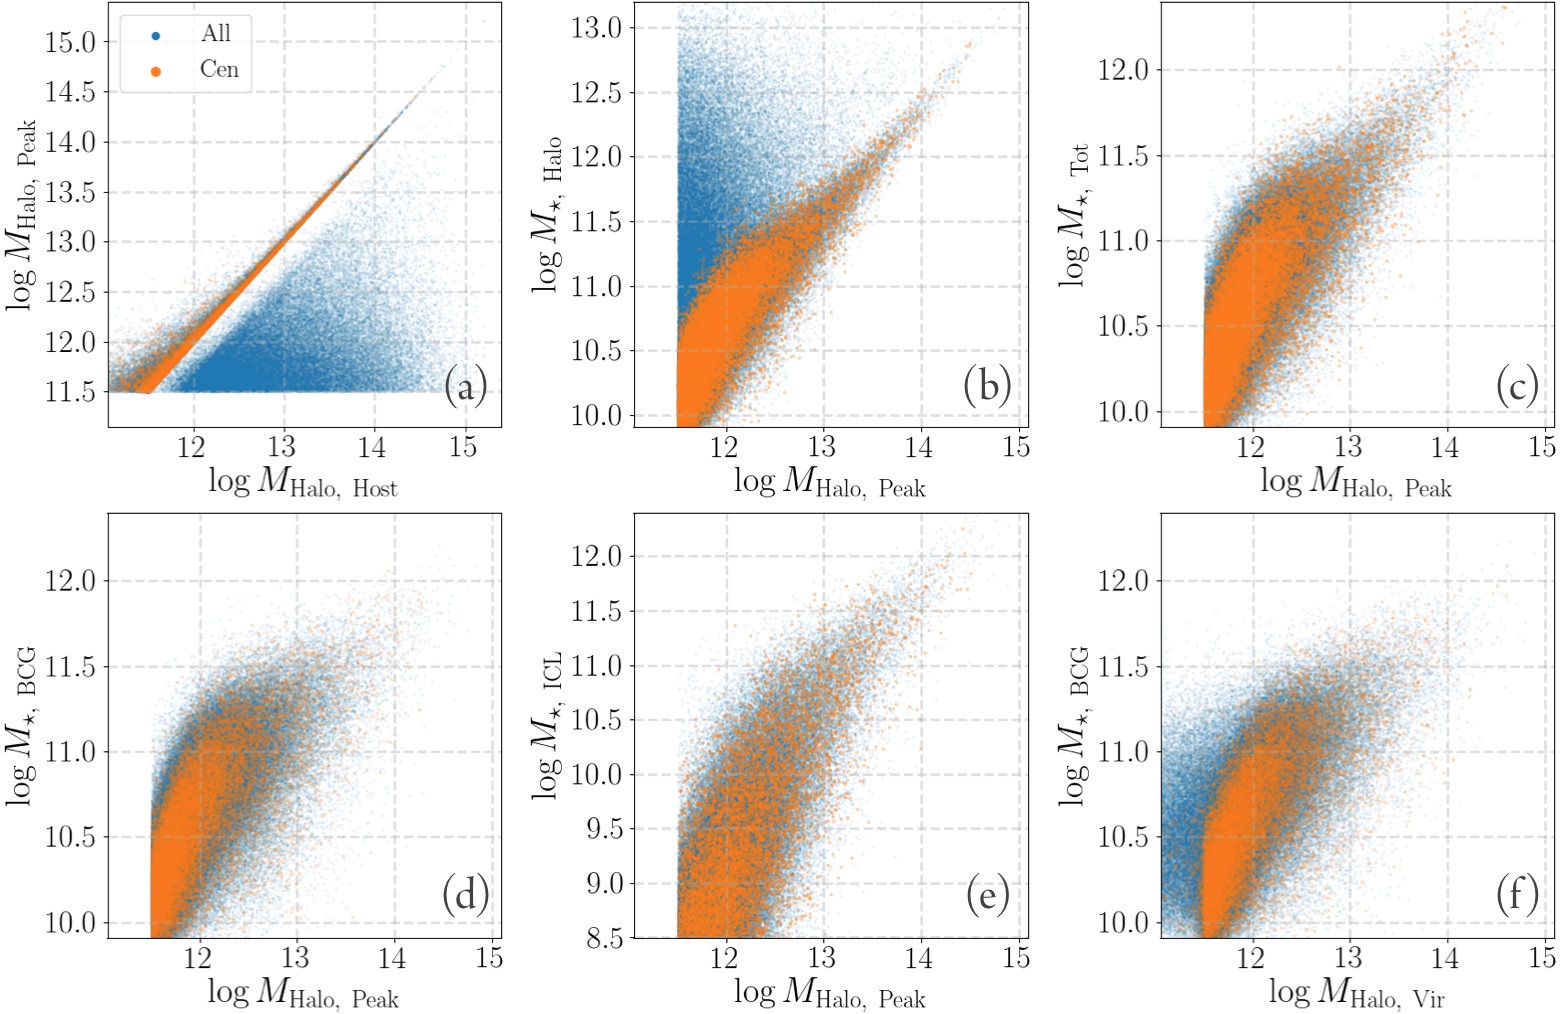
\includegraphics[width=\textwidth]{fig/um2_halo}
            \caption{
                Basic properties of the UniverseMachine model.  
                (a): The relationship between the host halo mass and the peak halo mass. 
                (b): Relation between peak halo mass and the stellar mass of all 
                galaxies within the halo; 
                (c): Relation between the peak halo mass and the total stellar mass 
                of the central galaxy system (BCG$+$ICL); 
                (d): Relation between peak halo mass and the BCG stellar mass; 
                (e): Relation between the peak halo mass and the ICL stellar mass; 
                (f): Relation between the Virial mass of the halo and the BCG stellar 
                mass.  
                Central galaxies are highlighted using orange color.
                }
        \label{fig:um2_halo}
    \end{figure*}
%% ------------------------------------------------------------------------------------ %% 

%% ------------------------------------------------------------------------------------ %% 
    \begin{figure*}
        \centering 
        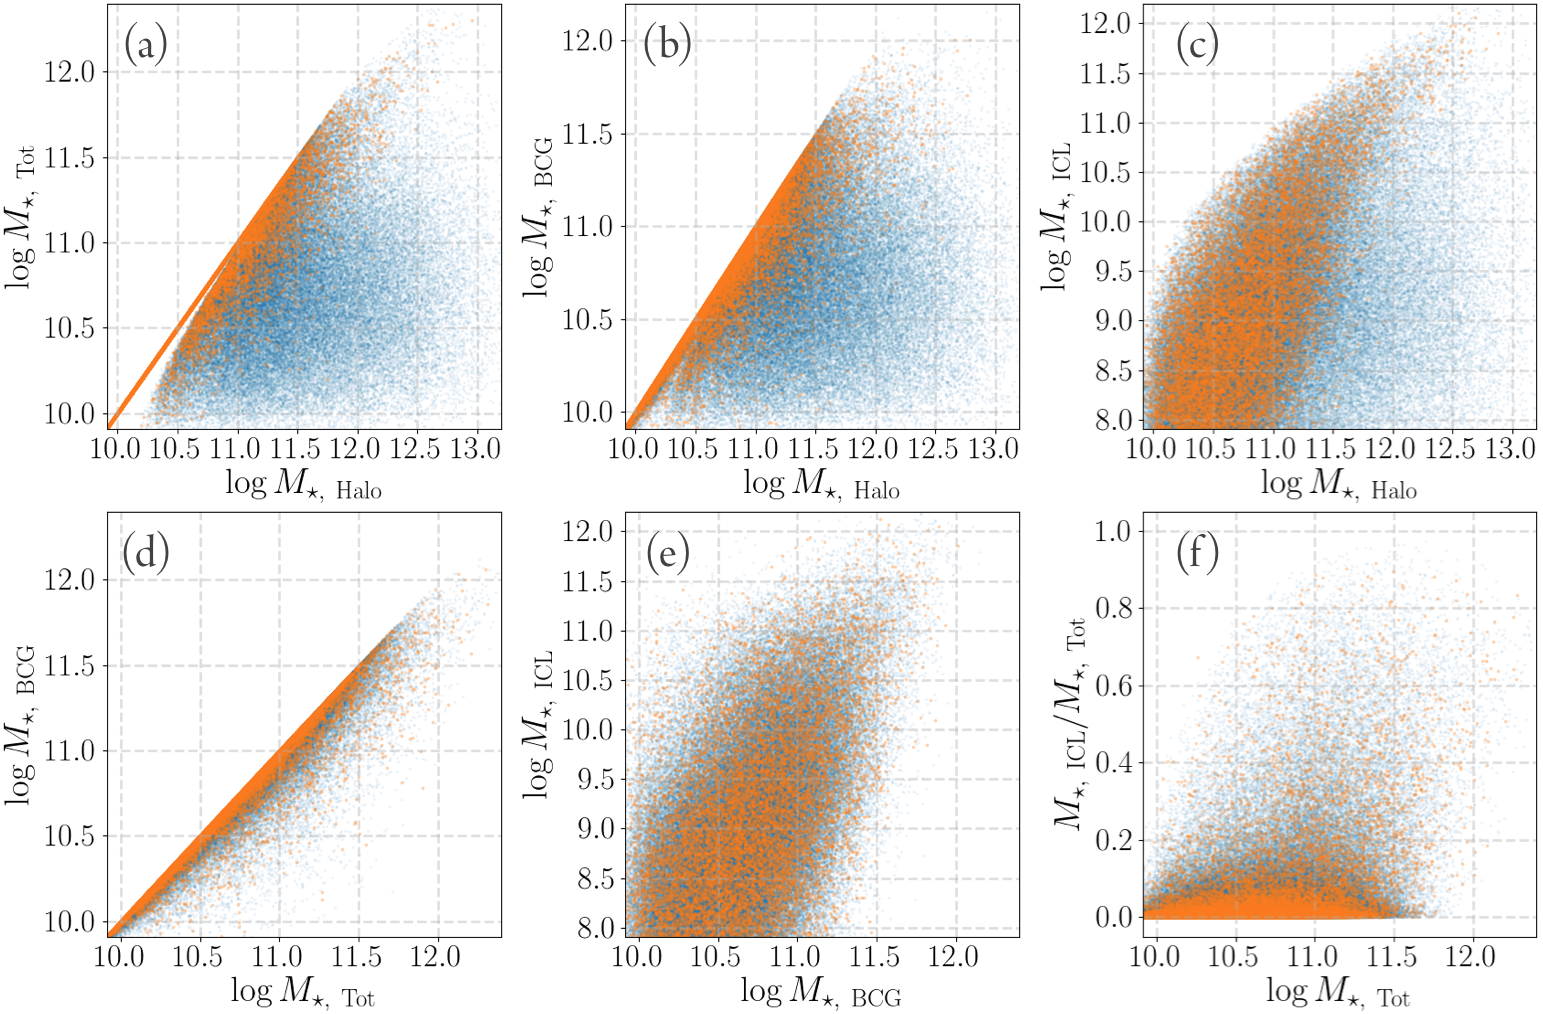
\includegraphics[width=\textwidth]{fig/um2_stellar}
            \caption{
                Relationships between different stellar masses in 
                UniverseMachine mock catalogs.  
                (a): All stellar masses in a halo and the total stellar mass of the 
                central galaxy system (BCG$+$ICL); 
                (b): All stellar mass in a halo and the stellar mass of the BCG; 
                (c): All stellar mass in a halo and the stellar mass of the ICL 
                component; 
                (d): Total stellar mass of the central galaxy system and the BCG 
                stellar mass; 
                (e): BCG stellar mass and the mass of the ICL component; 
                (f): Total stellar mass of the central galaxy system and the 
                fraction of ICL mass.  
                Central galaxies are highlighted using orange color.
                }
        \label{fig:um2_stellar}
    \end{figure*}
%% ------------------------------------------------------------------------------------ %% 


%% ------------------------------------------------------------------------------------ %% 
\subsection{\um{} Model}
    \label{ssec:um}
    
    \plan{Briefly explain the \um{} semi-empirical model.}


%% ------------------------------------------------------------------------------------ %% 
    \begin{figure*}
        \centering 
        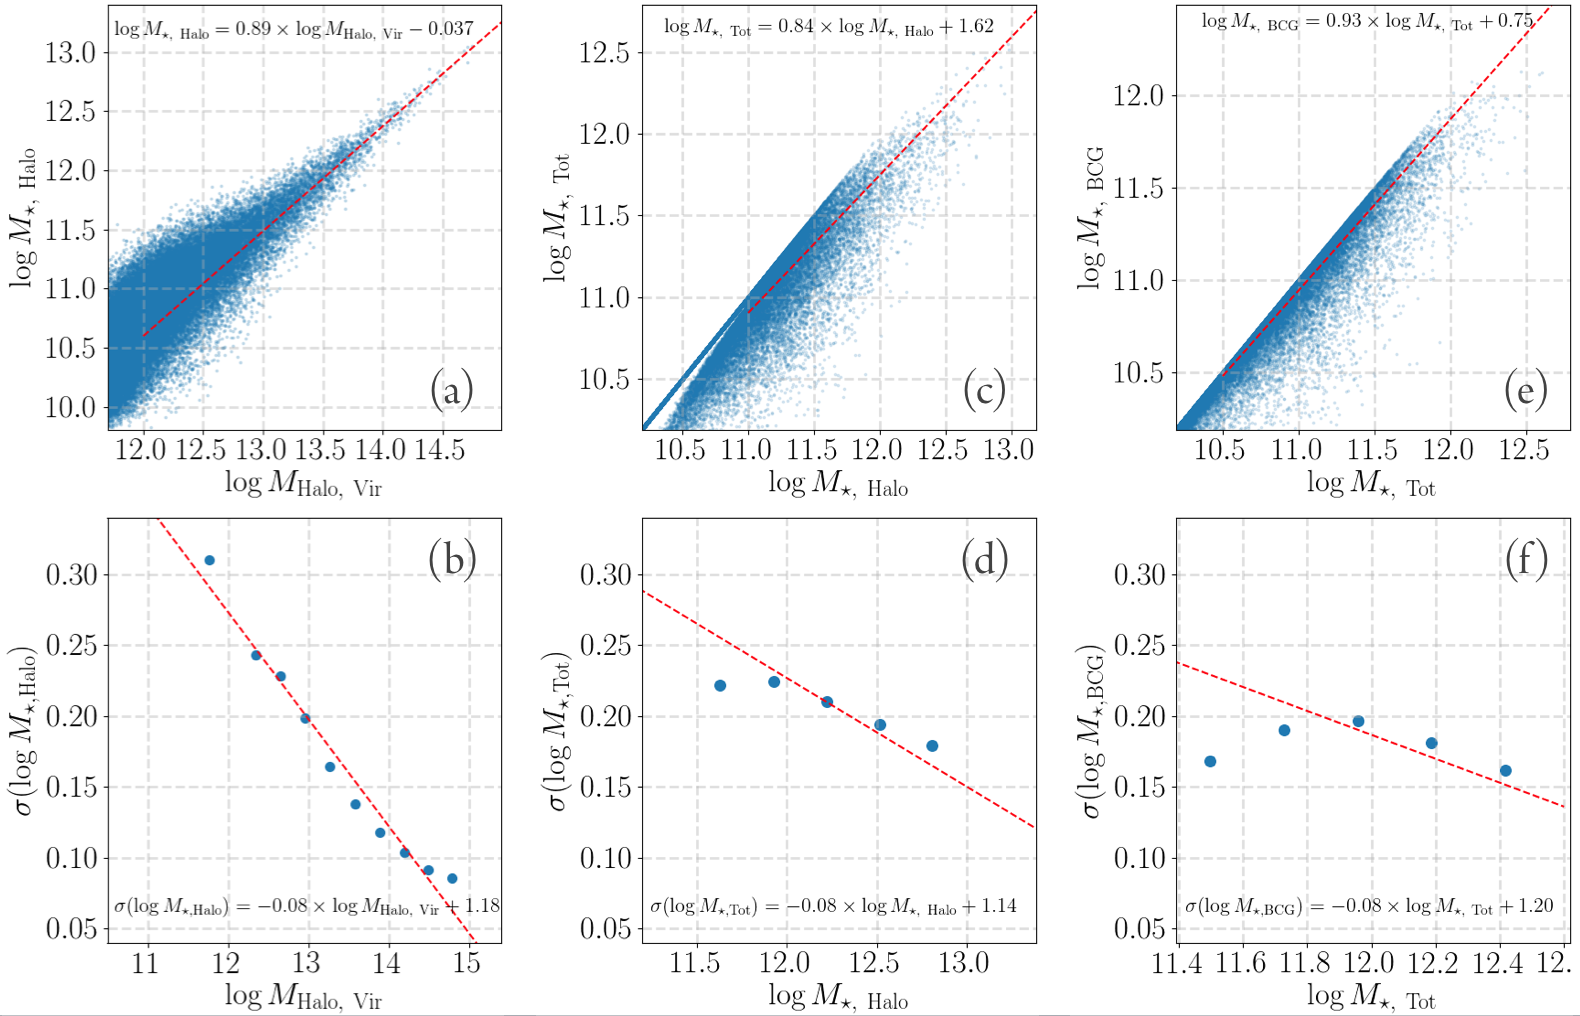
\includegraphics[width=\textwidth]{fig/um2_relation_initial}
            \caption{
                Simple log--log linear fit to some scaling relations in 
                \um{} mock catalogs.  
                These relations are for central galaxies only.  
                (a): Relation between the Virial halo mass and all stellar mass within 
                a halo; 
                (b) the scatters of total stellar mass in the halo in different halo 
                mass bins.  
                (c): Relation between all stellar mass in a halo and the total stellar 
                mass of the central galaxy system (BGC$+$ICL); 
                (d): the scatter of the total mass of the central galaxy.  
                (e): Relation between the total stellar mass of central galaxy system 
                and the BCG stellar mass; 
                (f): scatter of BCG stellar mass in different total stellar mass bins.   
                The red dashed-lines show the best--fit log--log linear relation.  
                The functional forms of these best--fit relations are also displayed.  
                The best--fit relations in panel (a) and (b) will be used as initial 
                guesses in our fit.
                }
        \label{fig:um2_stellar}
    \end{figure*}
%% ------------------------------------------------------------------------------------ %% 

%% ------------------------------------------------------------------------------------ %% 
\subsection{Old Model: the \mtot{}--\minn{} plane}
    \label{ssec:old_m100_m10}
    
    \plan{Need a lot of edits!}

    Physical motivation of this model is based on the finding in simulations that the 
    stellar mass of \emph{all} galaxies in the halo correlates the best with the 
    halo mass. 

    Here we describe the basic structure of the model. 
    The physical parameters used here are: 

    \begin{itemize}
    
        \item \mhalo{}: Mass of the dark matter halo. 
        \item \mall{}: Simulated/modelled stellar mass of all galaxies in the halo.
        \item \mbcg{}: Simulated/modelled stellar mass of the central part of the 
            galaxy.
        \item \micl{}: Simulated/modelled stellar mass of the intra-cluster light of 
            a halo. 
        \item \mcen{}: Simulated/modelled total stellar mass of the central galaxies. 
            Equals to \mbcg{}$+$\micl{}.
        \item \mtot{}: Observed stellar mass within a 100 kpc elliptical aperture. 
        \item \minn{}: Observed stellar mass within a 10 kpc elliptical aperture. 

    \end{itemize}
    
    Using the UniverseMachine model based on the MultiDark simulation (referred to 
    as the \um{} model), we assume there is a simple log--linear relation between 
    \mhalo{} and \mall{}: 

    \begin{equation}
        \log M_{\star,\ \mathrm{All}} = a \times \log M_{\rm Halo} + b 
    \end{equation}

    The above relation has a log--normal scatter.  
    The scatter varies with \mhalo{}, and follows a simple form: 

    \begin{equation}
        \sigma_{M_{\star,\ \mathrm{All}}} = c \times \log M_{\rm Halo} + d 
    \end{equation}

    And, the slopes and normalizations of these two simple relations ($a, b, c, d$) 
    are the four free parameters in this model.

    The other aspects of this model, including the predictions of stellar masses 
    within different radius, are simply inherited from the \um{} model. 
    We will ``remap'' the distributions of parameters using conditional abundance 
    matching method (provided by the \um{} software).  
    The original parameters from the UM2 model will be labelled with $\mathrm{Ori}$, 
    while the ``remapped'' ones will be labelled as $\mathrm{Remap}$.  

    To compare with observations, we make the assumption that, after the ``remapping'', 
    we can use the $M_{\star,\ \mathrm{Cen,\ Remap}}$ and 
    $M_{\star,\ \mathrm{BCG,\ Remap}}$ to match the observed \mtot{} and \minn{}.

    The ``remapped'' $M_{\star,\ \mathrm{Cen,\ Remap}}$ and 
    $M_{\star,\ \mathrm{BCG,\ Remap}}$ are from: 

    \begin{equation}
        M_{\star,\ \mathrm{Cen,\ Remap}} = M_{\star,\ \mathrm{All,\ Remap}} * 
            (M_{\star,\ \mathrm{Cen,\ Ori}} / M_{\star,\ \mathrm{All,\ Ori}})
    \end{equation}

    \begin{equation}
        M_{\star,\ \mathrm{BCG,\ Remap}} = M_{\star,\ \mathrm{Cen,\ Remap}} * 
            (M_{\star,\ \mathrm{BCG,\ Ori}} / M_{\star,\     \mathrm{Cen,\ Ori}})
    \end{equation}

    Here: 

    \begin{itemize}

        \item \fraccen{}: is the fraction of the stellar mass within a halo stored in 
            the central galaxy and the ICL components. 
            \fraccen{}$\sim 1.0$ means that central galaxy dominates the stellar mass 
            of the halo, and satellites make little contribution.
                
        \item \fracbcg{}: if we assume that the \mcen{} is the ``true'' total stellar 
            mass of the central galaxy system, \fracbcg{} is the fraction of the 
            stellar mass stored in the inner region of the central galaxy.
    
    \end{itemize}
    
    
    \plan{Describe the choices of models and how we perform the modelling (e.g., 
        details about the MCMC run).}

%% ------------------------------------------------------------------------------------ %% 
\subsection{New Model: the \mins{}--\macc{} plane}
    \label{ssec:new_m100_m10}

    \song{For discussion, we keep descriptions for both old and new models here.  
          Directly mapping the \mbcg{} and \mcen{} to our \minn{} and \mtot{}
          turns out to be problematic.  
          As show in the Figure~\ref{fig:um2_m100_m10_4}, the fraction of \mbcg{}
          in \mcen{} from the \um{} model shows a very different distribution 
          compared to the fraction of \minn{} in \mtot{} from HSC observations. 
          Too many \um{} massive galaxies have very high \mbcg{} fraction that 
          will significantly mislead the model. 
          \um{} model now uses a very simple model to determine the fraction of 
          stars that go into the ICL component after merger.  
          So it is not surprising that there is mismatch with observation. 
          }
          
    Here we describe the basic structure of the model. 
    The physical parameters used here are: 

    \begin{itemize}
    
        \item \mhalo{}: Dark matter halo mass. 
        
        \item \mall{}: Total stellar mass of all galaxies (central and satellites)
            in the dark matter halo.
        
        \item \mins{}: The stellar mass of the \insitu{} component, which is the 
            stars formed in the dark matter halo of the main progenitor.
        
        \item \macc{}: The stellar mass of the \exsitu{} component, which is the 
            stars accreted from merging with galaxies in other dark matter haloes. 
        
        \item \mgal{}: The total stellar mass of the galaxy, which is 
            \mins{}$+$\macc{}.
        
        \item \mtot{}: Observed stellar mass within a 100 kpc elliptical aperture. 
        
        \item \minn{}: Observed stellar mass within a 10 kpc elliptical aperture. 

    \end{itemize}

    Using the \um{} model based on the MultiDark simulation (referred to 
    as the \um{} model), we assume there is a simple log--linear relation between 
    \mhalo{} and \mall{}: 

    \begin{equation}
        \log M_{\star, \mathrm{All}} = a \times \log M_{\rm Halo} + b.
    \end{equation}

    The above relation has a log--normal scatter.  
    The scatter varies with \mhalo{}, and follows a simple form: 

    \begin{equation}
        \sigma_{\log{M_{\star, \mathrm{All}}}} = c \times \log M_{\rm Halo} + d.
    \end{equation}
    
    The slopes and normalizations of these two relations ($a, b, c, d$) will be 
    modelled as free parameters in our model.
    Using these assumptions, now we can `remap' the \um{} model to predict 
    the observed aperture stellar masses using conditional abundance matching 
    method. 
    This process makes use of two mass fractions from the \um{} model:
    
    \begin{itemize}
    
        \item $f_{\mathrm{Cen,\ UM}}=$\fraccen{}: 
            is the fraction of stellar mass of the central galaxy to the total 
            stellar mass within the halo. 
            $f_{\mathrm{Cen,\ UM}}\sim 1.0$ means that central galaxy dominates 
            the stellar mass budget of the halo.
                
        \item \fracbcg{}: if we assume that the \mcen{} is the ``true'' total stellar 
            mass of the central galaxy system, \fracbcg{} is the fraction of the 
            stellar mass stored in the inner region of the central galaxy.
 
    \end{itemize}
    
    In addition, we assume empirical relations between the modeled and observed 
    stellar masses. 
    
    In the simplest form, we assume the observed \minn{} represent a constant 
    fraction of the \insitu{} component, and \mtot{} represents the total stellar 
    mass of the galaxy: 
    
    \begin{align}
        \label{eqn:eqlabel}
        \begin{split}
        M_{\star, \mathrm{10\ kpc}} = f_{in-situ} \times M_{\star, in-situ},
        \\
        M_{\star, \mathrm{100\ kpc}} = M_{\star,\ in-situ} + M_{\star, ex-situ}.
        \end{split}
    \end{align}
    
    We will ``remap'' the distributions of parameters 
    using conditional abundance matching method.  
    The original parameters from the \um{} model will be labelled with $\mathrm{Ori}$, 
    while the ``remapped'' ones will be labelled as $\mathrm{Remap}$.  

    To compare with observations, we make the assumption that, after the ``remapping'', 
    we can use the $M_{\star,\ \mathrm{Cen,\ Remap}}$ and 
    $M_{\star,\ \mathrm{BCG,\ Remap}}$ to match the observed \mtot{} and \minn{}.

    The ``remapped'' $M_{\star,\ \mathrm{Cen,\ Remap}}$ and 
    $M_{\star,\ \mathrm{BCG,\ Remap}}$ are from: 

    \begin{equation}
        M_{\star,\ \mathrm{Cen,\ Remap}} = M_{\star,\ \mathrm{All,\ Remap}} * 
            (M_{\star,\ \mathrm{Cen,\ Ori}} / M_{\star,\ \mathrm{All,\ Ori}})
    \end{equation}

    \begin{equation}
        M_{\star,\ \mathrm{BCG,\ Remap}} = M_{\star,\ \mathrm{Cen,\ Remap}} * 
            (M_{\star,\ \mathrm{BCG,\ Ori}} / M_{\star,\     \mathrm{Cen,\ Ori}})
    \end{equation}

     

%% ------------------------------------------------------------------------------------ %% 
    \begin{figure*}
        \centering 
        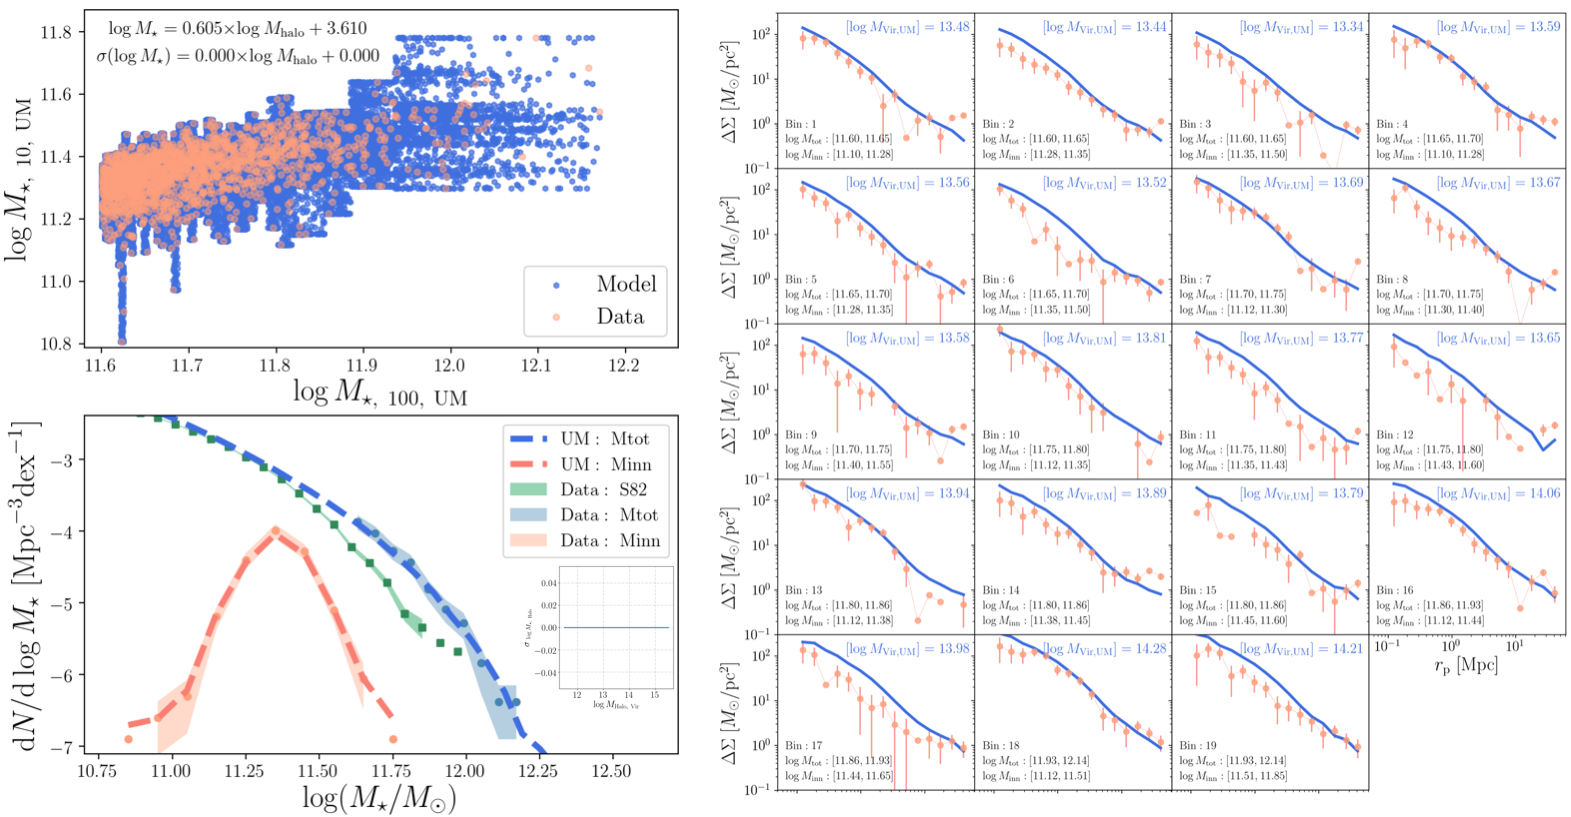
\includegraphics[width=\textwidth]{fig/um2_model_A}
            \caption{
                Overview of Model A 
                (Left): Distributions of the predicted stellar mass within 100 and 
                10 kpc, and comparisons with the observed stellar mass functions.  
                (Right): Comparisons between the predicted weak lensing mass density 
                profiles in different stellar mass bins and the observed ones in the 
                same bin.
                }
        \label{fig:um2_m100_m10_1}
    \end{figure*}
%% ------------------------------------------------------------------------------------ %% 

%% ------------------------------------------------------------------------------------ %% 
    \begin{figure}
        \centering 
        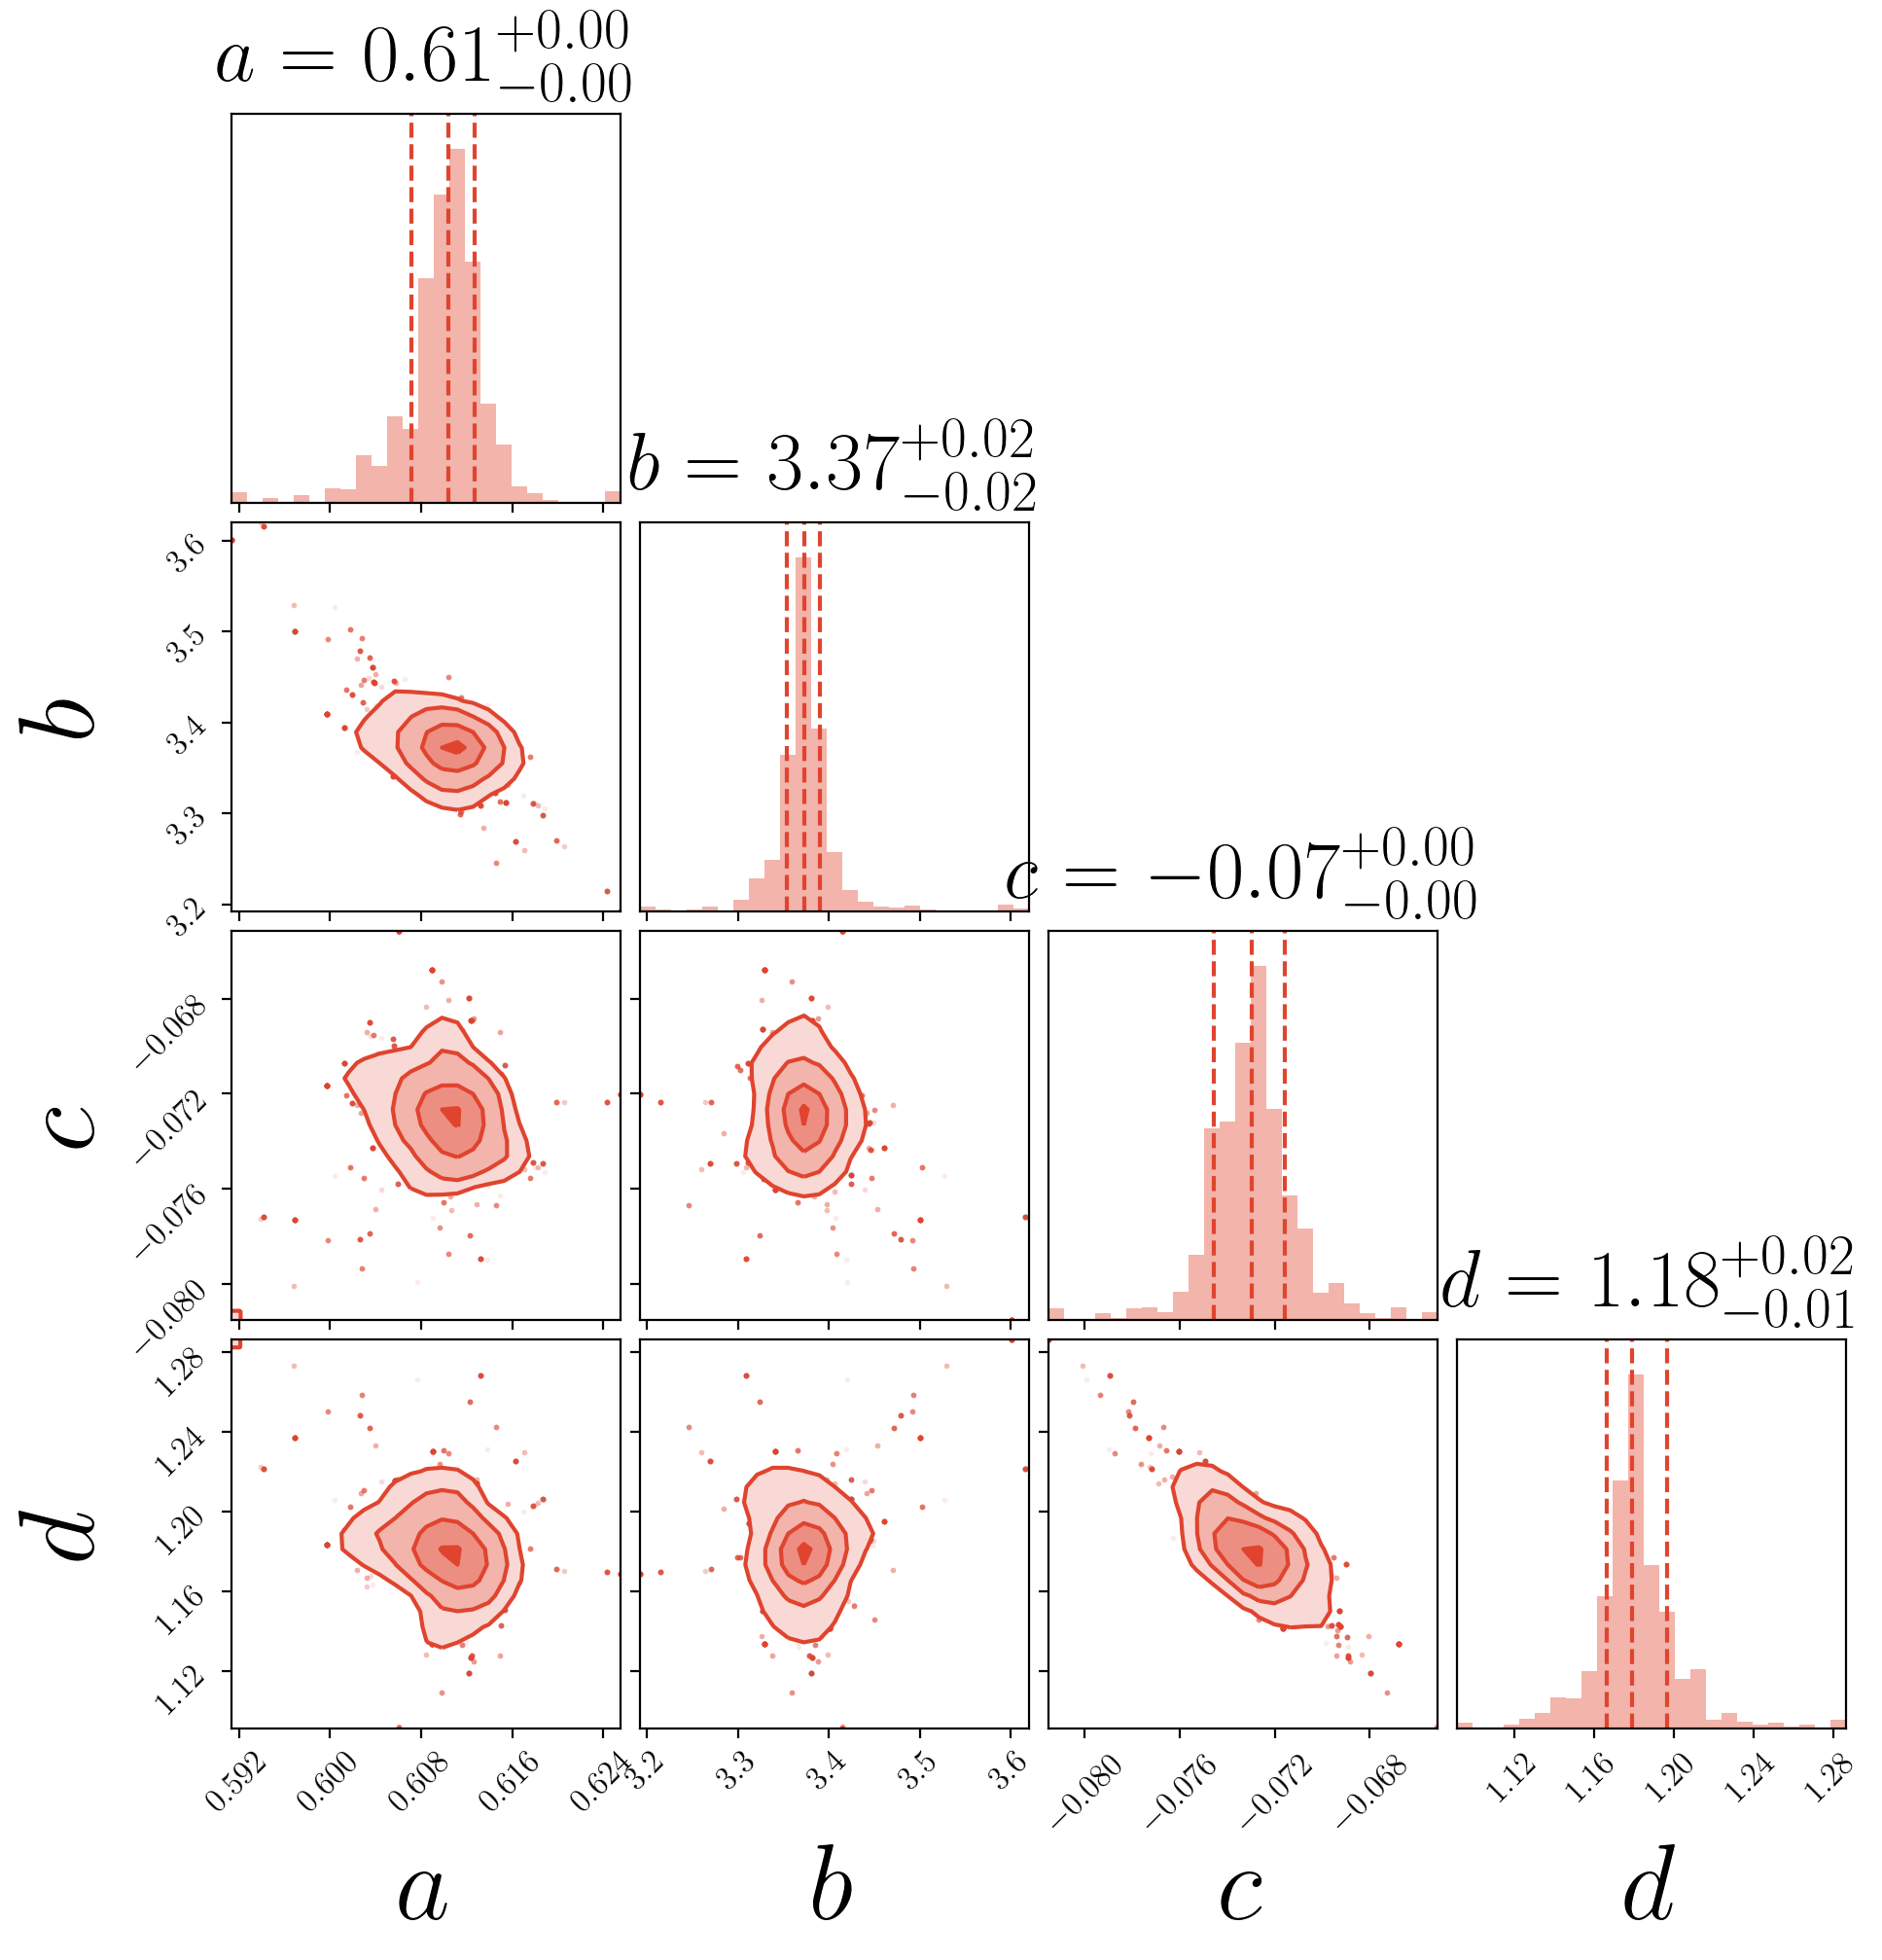
\includegraphics[width=\columnwidth]{fig/um2_model_A_corner}
            \caption{
                Corner plot for the best--fit parameters from the MCMC modelling.
                }
        \label{fig:um2_m100_m10_2}
    \end{figure}
%% ------------------------------------------------------------------------------------ %% 

%% ------------------------------------------------------------------------------------ %% 
\section{Results}
    \label{sec:result}

%% ------------------------------------------------------------------------------------ %% 
\subsection{Halo mass across the \mtot{}-\minn{} plane}
    \label{ssec:mhalo_wl}
    
    \plan{Key results: describe how does halo mass change across the \mtot{}-\minn{} 
          plane using the weak lensing signals.}

    \plan{Show similar trends in MassiveBlack-II simulation and in the \um{} model.}
          
%% ------------------------------------------------------------------------------------ %% 
\subsection{Results from forward modelling method}
    \label{ssec:m100_m10}
    
    \plan{Key results: describe how well the model can fit the stellar mass functions 
          and weak lensing signals at the same time, and what can we learn from the 
          best fit model.}

%% ------------------------------------------------------------------------------------ %% 
\section{Discussion}
    \label{sec:discussion}
    
    \begin{itemize}
        
        \item \plan{Caveats and limitations of this model}

        \item \plan{Implications on selecting galaxies using their central properties}
        
        \item \plan{Other scientific applications of this model}
                        
    \end{itemize}
%% ------------------------------------------------------------------------------------ %% 


%% ------------------------------------------------------------------------------------ %% 
\section{Summary and Conclusions}
    \label{sec:summary}
    
%% ------------------------------------------------------------------------------------ %% 
  
%% ------------------------------------------------------------------------------------ %% 
%% ------------------------------- Acknowledgements ----------------------------------- %% 
%% ------------------------------------------------------------------------------------ %% 

\section*{Acknowledgements}

  % HSC part
  The Hyper Suprime-Cam (HSC) collaboration includes the astronomical communities of 
  Japan and Taiwan, and Princeton University.  The HSC instrumentation and software were
  developed by the National Astronomical Observatory of Japan (NAOJ), the Kavli Institute
  for the Physics and Mathematics of the Universe (Kavli IPMU), the University of Tokyo,
  the High Energy Accelerator Research Organization (KEK), the Academia Sinica Institute
  for Astronomy and Astrophysics in Taiwan (ASIAA), and Princeton University.  
  Funding was contributed by the FIRST program from Japanese Cabinet Office, the Ministry 
  of Education, Culture, Sports, Science and Technology (MEXT), the Japan Society for 
  the Promotion of Science (JSPS), Japan Science and Technology Agency (JST), the
  Toray Science Foundation, NAOJ, Kavli IPMU, KEK, ASIAA, and Princeton University.
   
  % SDSS part
  Funding for SDSS-III has been provided by the Alfred P. Sloan Foundation, the
  Participating Institutions, the National Science Foundation, and the U.S.  Department of
  Energy. The SDSS-III web site is http://www.sdss3.org.  SDSS-III is managed by the
  Astrophysical Research Consortium for the Participating Institutions of the SDSS-III
  Collaboration including the University of Arizona, the Brazilian Participation Group,
  Brookhaven National Laboratory, University of Cambridge, University of Florida, the
  French Participation Group, the German Participation Group, the Instituto de Astrofisica
  de Canarias, the Michigan State/Notre Dame/JINA Participation Group, Johns Hopkins
  University, Lawrence Berkeley National Laboratory, Max Planck Institute for
  Astrophysics, New Mexico State University, New York University, Ohio State University,
  Pennsylvania State University, University of Portsmouth, Princeton University, the
  Spanish Participation Group, University of Tokyo, University of Utah, Vanderbilt
  University, University of Virginia, University of Washington, and Yale University.
  
  % Pan-STARRS1 part
  The Pan-STARRS1 Surveys (PS1) have been made possible through contributions of the 
  Institute for Astronomy, the University of Hawaii, the Pan-STARRS Project Office, 
  the Max-Planck Society and its participating institutes, the Max Planck Institute 
  for Astronomy, Heidelberg and the Max Planck Institute for Extraterrestrial Physics, 
  Garching, The Johns Hopkins University, Durham University, the University of Edinburgh, 
  Queen's University Belfast, the Harvard-Smithsonian Center for Astrophysics, the Las 
  Cumbres Observatory Global Telescope Network Incorporated, the National Central 
  University of Taiwan, the Space Telescope Science Institute, the National Aeronautics 
  and Space Administration under Grant No. NNX08AR22G issued through the Planetary 
  Science Division of the NASA Science Mission Directorate, the National Science 
  Foundation under Grant No. AST-1238877, the University of Maryland, and Eotvos 
  Lorand University (ELTE).
  
  % LSST software
  This paper makes use of software developed for the Large Synoptic Survey 
  Telescope. We thank the LSST Project for making their code available as free 
  software at http://dm.lsstcorp.org.
 
  % Software
  This research made use of:
  \href{http://www.stsci.edu/institute/software_hardware/pyraf/stsci\_python}{\texttt{STSCI\_PYTHON}},
      a general astronomical data analysis infrastructure in Python. 
      \texttt{STSCI\_PYTHON} is a product of the Space Telescope Science Institute, 
      which is operated by AURA for NASA;
  \href{http://www.scipy.org/}{\texttt{SciPy}},
      an open source scientific tools for Python (\citealt{SciPy});
  \href{http://www.numpy.org/}{\texttt{NumPy}}, 
      a fundamental package for scientific computing with Python (\citealt{NumPy});
  \href{http://matplotlib.org/}{\texttt{Matplotlib}}, 
      a 2-D plotting library for Python (\citealt{Matplotlib});
  \href{http://www.astropy.org/}{\texttt{Astropy}}, a community-developed 
      core Python package for Astronomy (\citealt{AstroPy}); 
  \href{http://scikit-learn.org/stable/index.html}{\texttt{scikit-learn}},
      a machine-learning library in Python (\citealt{scikit-learn}); 
  \href{http://www.astroml.org/}{\texttt{astroML}}, 
      a machine learning library for astrophysics (\citealt{astroML});
  \href{https://ipython.org}{\texttt{IPython}}, 
      an interactive computing system for Python (\citealt{IPython});
  \href{https://github.com/kbarbary/sep}{\texttt{sep}} 
      Source Extraction and Photometry in Python (\citealt{PythonSEP});
  \href{https://jiffyclub.github.io/palettable/}{\texttt{palettable}},
      color palettes for Python;
  \href{http://dan.iel.fm/emcee/current/}{\texttt{emcee}}, 
      Seriously Kick-Ass MCMC in Python;
  \href{http://bdiemer.bitbucket.org/}{\texttt{Colossus}}, 
      COsmology, haLO and large-Scale StrUcture toolS (\citealt{Colossus}).

%% ------------------------------------------------------------------------------------ %% 
%% ----------------------------- Bibliographic Section -------------------------------- %% 
%% ------------------------------------------------------------------------------------ %% 

\bibliographystyle{mnras}
\bibliography{galaxy_halo}

%% ------------------------------------------------------------------------------------ %% 
%% Table.1 
%% ------------------------------------------------------------------------------------ %% 
%\clearpage
%\include{table1}
%\clearpage
%% ------------------------------------------------------------------------------------ %% 

%% ------------------------------------------------------------------------------------ %% 
%% ------------------------------------ Appendix -------------------------------------- %% 
%% ------------------------------------------------------------------------------------ %% 

\appendix

%% ------------------------------------------------------------------------------------ %% 
\section{Details about sample selection} 
	\label{app:sample} 

%% ------------------------------------------------------------------------------------ %% 
\section{Details about sed fitting} 
	\label{app:sed} 

%% ------------------------------------------------------------------------------------ %% 
\section{Details about aperture mass estimates} 
	\label{app:sed} 
	
%% ------------------------------------------------------------------------------------ %% 
\section{Details about the \um{} model} 
	\label{app:model} 

%% ------------------------------------------------------------------------------------ %% 
    \begin{figure}
        \centering 
        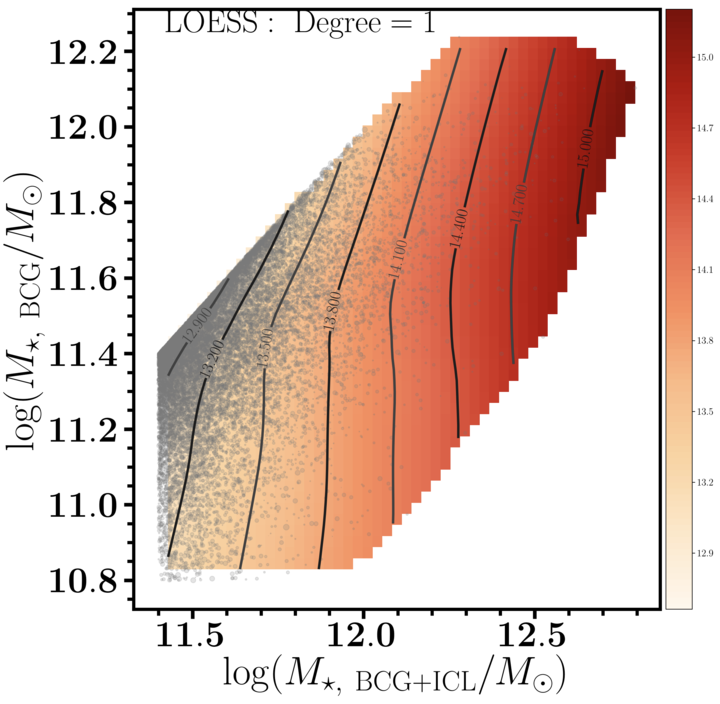
\includegraphics[width=\columnwidth]{fig/um2_tot_bch_halo}
            \caption{
                The relationship between the total stellar mass of the central galaxies 
                and the BCG stellar masses from the \um{} mock catalogs.  
                The continuous color surface shows the smooth maps of halo mass using 
                degree$=1$ \texttt{LOESS} method (Locally Weighted Regression, 
                Cleveland 1979, Cleveland \& Devlin 1988, \citealt{Cappellari2013b}).  
                The `iso--\mhalo{}' curves are overlaid as well.
                }
        \label{fig:um2_m100_m10_3}
    \end{figure}
%% ------------------------------------------------------------------------------------ %% 

%% ------------------------------------------------------------------------------------ %% 
    \begin{figure*}
        \centering 
        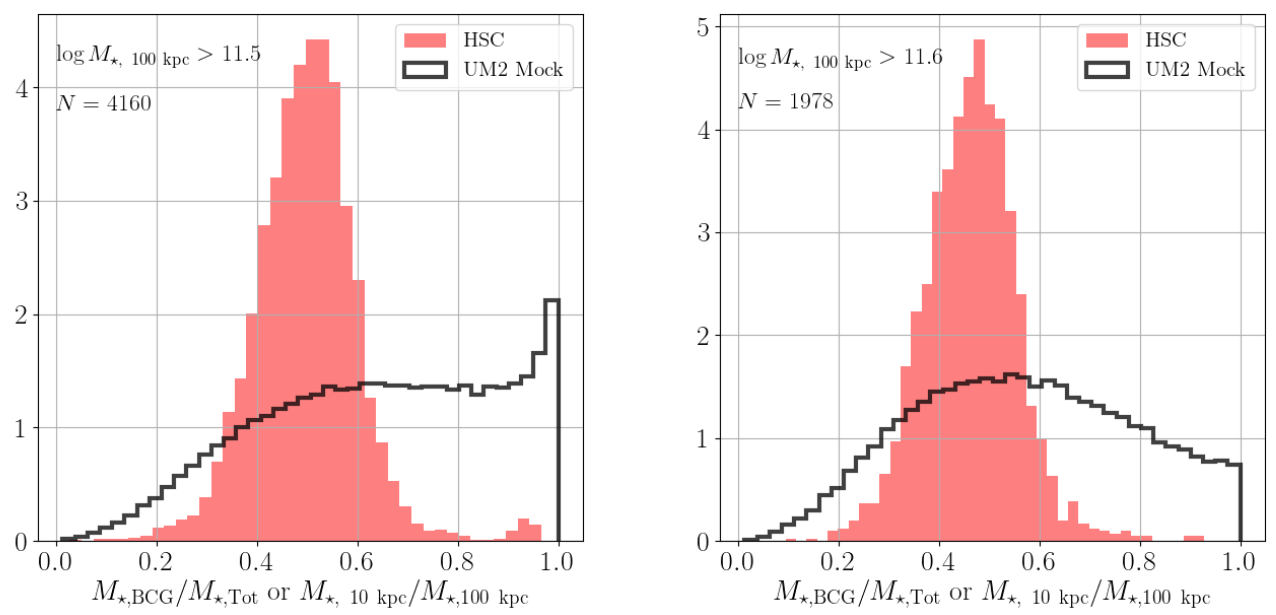
\includegraphics[width=\textwidth]{fig/um2_mbcg_mtot_frac}
            \caption{
                Comparisons between the fraction of BCG stellar mass in the BCG$+$ICL 
                central galaxy system from UniverseMachine mock catalog and the 
                fractional ratio between stellar mass within 10 and 100 kpc from HSC 
                observations.  
                The HSC data are at $0.3 < z < 0.5$.  
                We pick two subsamples with the stellar mass within 100 kpc apertures 
                larger than $10^{11.5} M_{\odot}$ (Left panel, 4160 galaxies) and 
                $10^{11.6}$ (Right panel, 1978 galaxies) solar mass.  
                We pick massive galaxies from the \um{} mock catalogs above the same 
                volume density.  
                We can see that the two distributions are quite different.  
                The \um{} distributions have a higher average fraction and much 
                larger scatter.  
                And there appears to be a population of central galaxies in \um{} with 
                no ICL component at all, especially in the left sample.
                }
        \label{fig:um2_m100_m10_4}
    \end{figure*}
%% ------------------------------------------------------------------------------------ %% 

%% ------------------------------------------------------------------------------------ %%  
\bsp
\label{lastpage}
\end{document}
%% ------------------------------------------------------------------------------------ %% 